\cleardoublepage

\chapter{Propuesta}
\label{ch:Capitulo3}

Tras presentar diferentes tecnologías, software, protocolos de comunicación y hardware planteados en el ámbito de la domótica del hogar del capitulo Chapter~\ref{ch:Capitulo2}, en la búsqueda de una solución libre y de bajo coste, que pueda alcanzar los objetivos planteados para la creación de un prototipo de suite domótica, se propone:

\vspace{1cm}

Desarrollar un prototipo de suite domótica que opere en una red local inalámbrica cuyo router actúe como nodo principal, ejecutado en un ordenador de bajo consumo, que permita la interconexión para dispositivos inalámbricos con roles de actuadores o sensores. Además, debe ser posible operar dicha suite, desde dentro de la red local en la que opera el nodo, o desde fuera de la misma mediante conexiones remotas cifradas, mediante una aplicación para dispositivo móvil con sistema operativo Android. Si bien, la operatividad remota es opcional, se debe alcanzar la gestión de la suite en el entorno de la red local, cumpliendo así con el objetivo de disponer de un sistema aislado y autónomo, que no dependa de servicios externos para su funcionamiento. Una vez alcanzada una implementación funcional del prototipo se aplicará en dos casos de usos que ejemplifican la entrada y salidas características de todo sistema de domótica, la recepción, proceso y presentación de datos de un dispositivo sensor en la aplicación móvil, y la gestión de un actuador desde dicha aplicación. Esta suite debe cubrir la necesidad de controlar el estado de una bodega de uso personal en una casa, pudiendo obtener valores ambientales de la estancia y controlar el sistema de iluminación de la escalera que accede a la misma, pudiendo alternar el estado de las luces de manera automática o manualmente, desde la aplicación. 

\vspace{1cm}

Adicionalmente se tratará de alcanzar una cierta descentralización de los dispositivos y la propia Raspberry, basándose en el concepto de nodo principal (gateway), que habitualmente se observa en las plataformas de pago. Para lograr la propuesta, será necesario considerar de entre las opciones estudiadas en el  Chapter~\ref{ch:Capitulo2} aquellas que se ajustan mejor al alcance de esta propuesta. Dadas las distintas capas de hardware, arquitectura de red y software que componen este proyecto, la propuesta será dividida en tres conceptos modulares, permitiendo un desarrollo individual y en paralelo respecto de cada uno.

Se ha elegido no utilizar un \gls{framework} concreto para el desarrollo de nuestra suite domótica en la parte que gestiona, queda a nuestra entera disposición seleccionar, bajo que servicios operará nuestra solución domótica. Cualquiera de los \gls{framework} anteriormente listados estaban sujetos a una combinación de servicios que les permitía operar dentro de sus especificaciones. En más de la mitad de ellos, se utilizaban servidores web que permitan gestionar la suite domótica vía web, o a través de una \gls{app}.

Dichos planteamientos se basan en que todo sensor/actuador que forme parte de red de dispositivos de una solución de domótica actual, es gestionada a través de un nodo. En vez de conectar los dispositivos inalámbricos a el router de la casa, se conectan al nodo y este, a su vez, es quien se conecta a la red local del hogar, para así conectarse con los servicios externos. En general, las distintas plataformas has alcanzado un acuerdo no formalizado de actuación que funciona de la siguiente forma. El usuario final compra un nuevo dispositivo, lo enciende, dejándolo en un estado de "inclusión" a la red domótica, después, desde la aplicación de móvil, se indica al nodo, que se quiere añadir un nuevo dispositivo, y tras seguir las indicaciones, el dispositivo se registra en la red del nodo. Esto, sin embargo, tiene algunos inconvenientes en el proceso de "inclusión", y aunque la probabilidad es baja, puede suceder que dos nodos de distintas viviendas, que están registrando dispositivos simultáneamente, terminasen, registrando un dispositivo que no les corresponde. Esto es una vulnerabilidad de seguridad grave y una vertiente adicional que incluir en las motivaciones del estudio y desarrollo de una suite domótica libre que permita nuevas formulas de funcionamiento.

Se ha planteado este problema, junto con las 3 motivaciones principales, para crear un proceso de "inclusión" de dispositivos al nodo, que parta de una conexión alámbrica (vía USB) y resuelva este inconveniente, y simplifique el proceso de las soluciones privadas, que en ocasiones pueden fallar.

Podría parecer que hablamos de una relación de objetos entre sí, y que un modelo de \gls{bbdd} relacional es la mejor opción, pero si consideramos que, cada entrada almacenada tendrá una estructura distinta, hace que no sea una opción tan ideal. Pensemos, por ejemplo, que utilizando una \gls{bbdd} SQL se planifica un conjunto de tablas relacionadas entre sí. Sera necesaria una tabla que contenga las ubicaciones y se relacione con otra tabla que definan a los dispositivos. Esto establece una relación 1:N donde múltiples dispositivos pueden existir para una estancia, pero nunca en varias a la vez. De cada dispositivo existirá una nueva relación 1:N de medidas. Lo cual deja un esquema semejante al de la figura siguiente:


\begin{figure}[hbt!]
\centering
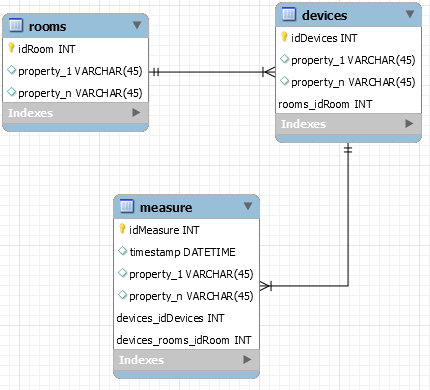
\includegraphics[height=2.5in]{figures/SQLSchemaExample_1.png}
\end{figure}

\vspace{1.5cm}

Sin embargo, existen algunos problemas graves de diseño de esta idea, en primer lugar, los dispositivos no pueden ser una propiedad de una estancia. Son objetos relacionados, pero no existe una transitividad dura entre ellos. Un dispositivo puede cambiar de estancia en un momento dado, y aun asi, seguir existiendo medidas en fechas concretas de ese dispositivo para una habitación en la cual, dicho dispositivo ya no está relacionado. Otro posible escenario es la desaparición de una estancia (como resultado de fusionar 2 estancias en una al derribar una pared). Para mantener una integridad lógica y persistente a lo largo del tiempo. Toda medida deberá tener un campo que determine en que ubicación fue tomada.
no hay transitividad dura entre room y device, lo cual hace que sean independientes entre sí.


\begin{figure}[hbt!]
\centering
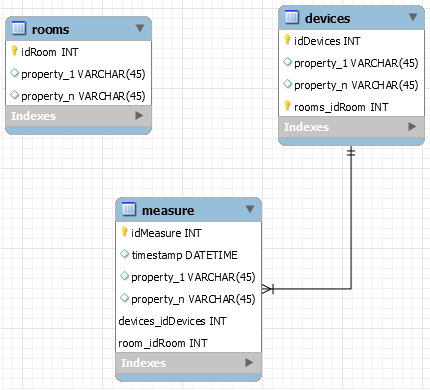
\includegraphics[height=2.5in]{figures/SQLSchemaExample_2.png}
\end{figure}

\vspace{1.5cm}

Con esto aún tendríamos que enfrentar un problema adicional, el número de columnas que definen las propiedades de una tabla. El ejemplo más claro es la tabla de medidas. Una medida, efectuada por un sensor será definida por su identificador y la fecha en la que se realizó, ahora bien, según la naturaleza del dispositivo, se obtendrán disantos tiempos de medida. Un sensor combinado de temperatura y humedad nos dará dos magnitudes de medición, un sensor de ruido almacenará un valor de decibelios, una luz define su medida por su estado de actividad (encendido o apagado), aunque por otra parte podría indicar el consumo eléctrico, o propiedades adicionales como intensidad de luz, o incluso color. Es cierto que, para un actuador, como lo es un emisor de luz, no realiza medidas como tal, y sus correspondientes estados de actividad podrían ser más adecuados definirlos como propiedades del dispositivo y no como medidas. Podríamos separar las medidas de los estados en tablas distintas, pero igualmente llegaríamos al problema del número de campos necesarios en una tabla. Valor que por otra parte es muy difícil de prever en base a la extensa gama de dispositivos existentes. Esto puede solucionarse de manera sencilla con 2 estrategias. Incluir una gran cantidad de columnas en previsión de los distritos tipos de medidas existentes, dejando que las medidas posean un valor nulo para los campos no utilizados en función de la relación de su sensor, o bien, unificar todos los campos en un único valor de cadena de caracteres que almacene un dato estructurado, como es el caso de los JSON. Esta última opción, sería la más deseable tanto por sencillez de implementación como facilidad de procesamiento. Lo que dejaría un esquema semejante a este:

\begin{figure}[hbt!]
\centering
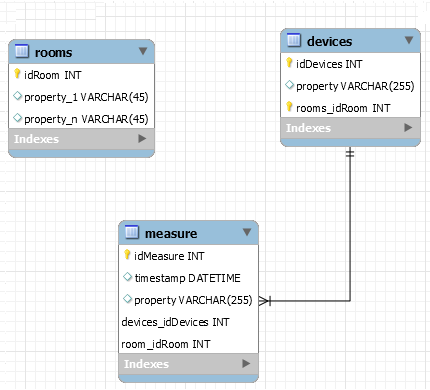
\includegraphics[height=2.5in]{figures/SQLSchemaExample_3.png}
\end{figure}

Una preocupación que agrava la perspectiva de usar una \gls{bbdd} relacional es, en este punto del proyecto, su escalabilidad horizontal. Si bien las tablas pueden crecer a un gran número de registros, no se prevé almacenar datos con vistas a largo plazo, la mayoría de los valores almacenados serán efímeros en tiempo de utilidad, almacenarlos responde solo a la necesidad de obtener comparativas en plazos de tiempo relativamente cortos, como horas, días, y posiblemente semanas. Mas allá de este rango estos datos no tienen una utilidad real y pueden ser condensados en medidas para utilizarse en resúmenes. Por otro lado, disponer de flexibilidad a la hora de configurar la extensión de propiedades de un objeto de la \gls{bbdd} es uno de los puntos fuertes de una \gls{bbdd} no relacional.

\vspace{1.5cm}


\section{Módulos de la propuesta}
\label{ch:Capitulo3.2}

Se creará un nodo principal que actuara como router de la red de dispositivos de la suite domótica y servidor de la aplicación móvil. Dispondrá de la capacidad de ser operado de forma remota o local, almacenara los servicios y aplicaciones necesarios para que funcione la suite domótica ejecutándose en un ordenador de bajo consumo.

Se genera distintos dispositivos sensores o actuadores que podrán incluirse en la red inalámbrica del nodo principal y podrán ser operados desde dicho nodo.

Y por último la aplicación movil (front-end) y servidor (back-end) que darán al usuario la capacidad de gestionar la suite domótica.

\section{Propuesta de casos de uso}
\label{ch:Capitulo3.3}

El primer caso de uso consistirá en una simple interacción del usuario con la suite domótica para consultar la temperatura y/o humedad de una estancia. Para ello, es necesario disponer de un dispositivo inalámbrico con un sensor que recoja las mediciones y puedan ser mostradas al usuario en su smartphone.

El segundo caso de uso cubrirá la gestión por parte del usuario de un actuador basado en un interruptor de corriente, pudiendo consultar su estado actual y alternar dicho estado, también desde un smartphone.

\section{Objetivos adicionales}
\label{ch:Capitulo3.4}

Las siguientes propuestas corresponden más a un declaración de intenciones que a objetivos necesarios para cumplir la propuesta del proyecto. Son un valor añadido y deseable siempre que no comprometan los plazos de tiempo marcados por la entrega final de este documento al director de proyecto. Se encuentran enumerados según el valor de importancia.

\begin{enumerate}

  \item Vinculación de dispositivos con la red de suite domótica mediante USB, en lugar del clásico emparejamiento WIFI.

  \item Creación de una imagen autoinstalable de para otros usuarios

  \item Integración de múltiples opciones de hardware compatibles con la suite domótica.

  \item Conexiones cifradas en la red de dispositivos y en la comunicación entre aplicación movil y servidor.

  \item Exportar la suite domótica en una imagen autoinstalable, de fácil instalación que permita replicar el prototipo creado.

\end{enumerate}

\begin{figure}[hbt!]
\centering
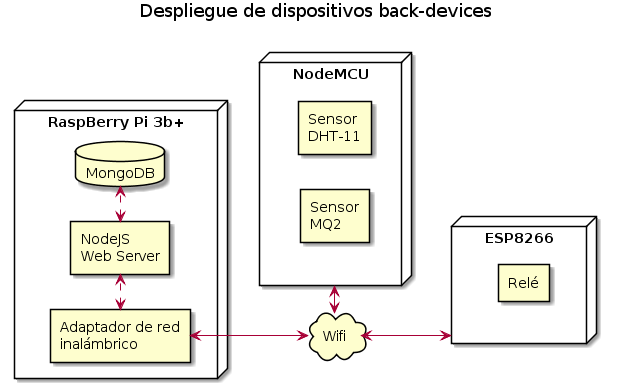
\includegraphics[height=2.5in]{figures/diagrams/physical-devices/back-devices.png}
\caption[back-devices]{back-devices\footnotemark}
\end{figure}

\begin{figure}[hbt!]
\centering
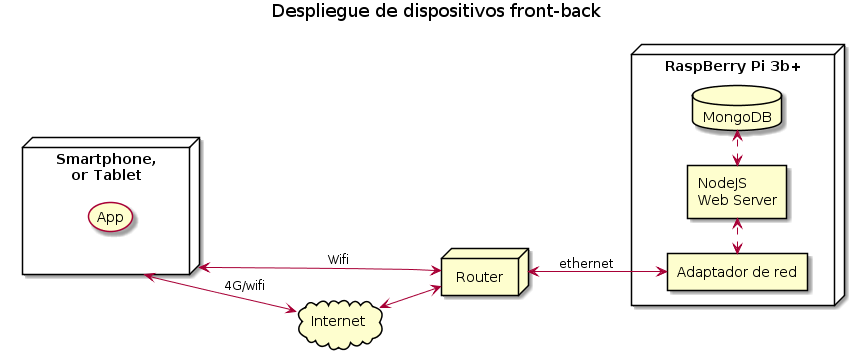
\includegraphics[height=2.5in]{figures/diagrams/physical-devices/front-back.png}
\caption[front-back]{front-back\footnotemark}
\end{figure}

\begin{figure}[hbt!]
\centering
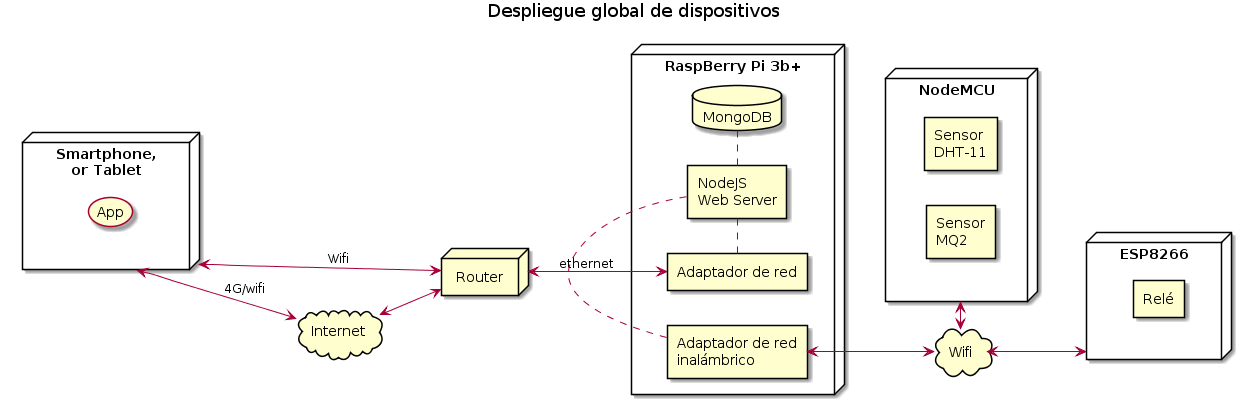
\includegraphics[height=2.5in]{figures/diagrams/physical-devices/global.png}
\caption[global]{global\footnotemark}
\end{figure}

\begin{figure}[hbt!]
\centering
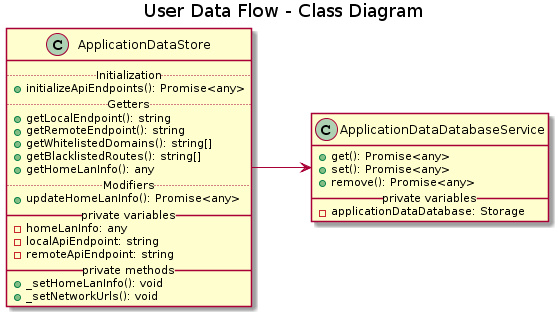
\includegraphics[height=2.5in]{figures/diagrams/front/data-flow/app-data.png}
\caption[app-data]{app-data\footnotemark}
\end{figure}

\begin{figure}[hbt!]
\centering
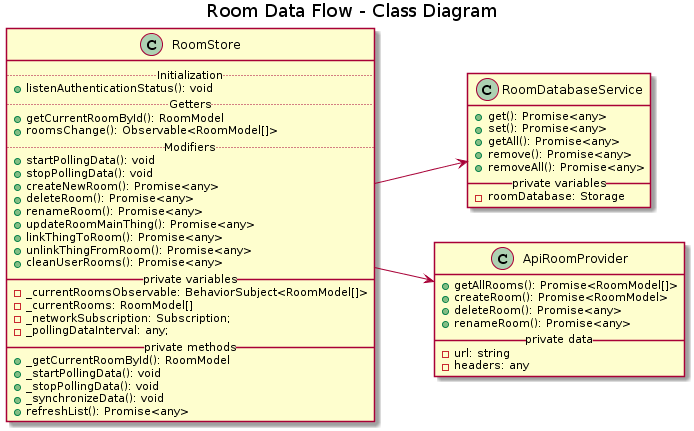
\includegraphics[height=2.5in]{figures/diagrams/front/data-flow/room.png}
\caption[room]{room\footnotemark}
\end{figure}

\begin{figure}[hbt!]
\centering
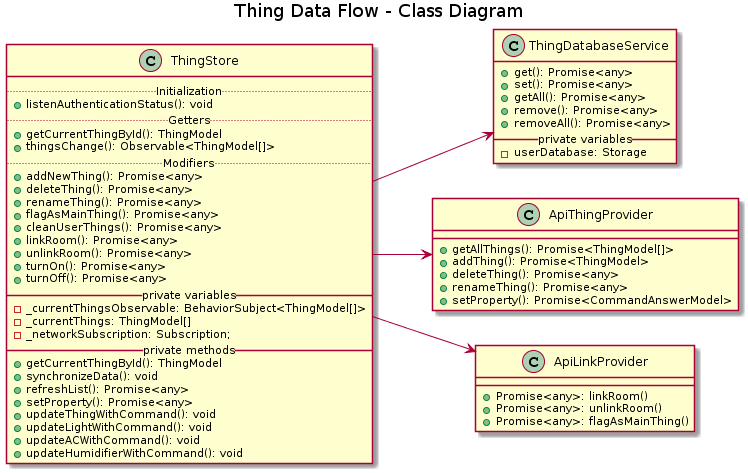
\includegraphics[height=2.5in]{figures/diagrams/front/data-flow/thing.png}
\caption[thing]{thing\footnotemark}
\end{figure}

\begin{figure}[hbt!]
\centering
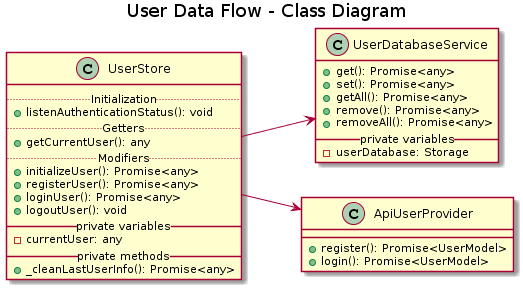
\includegraphics[height=2.5in]{figures/diagrams/front/data-flow/user.png}
\caption[user]{user\footnotemark}
\end{figure}

\begin{figure}[hbt!]
\centering
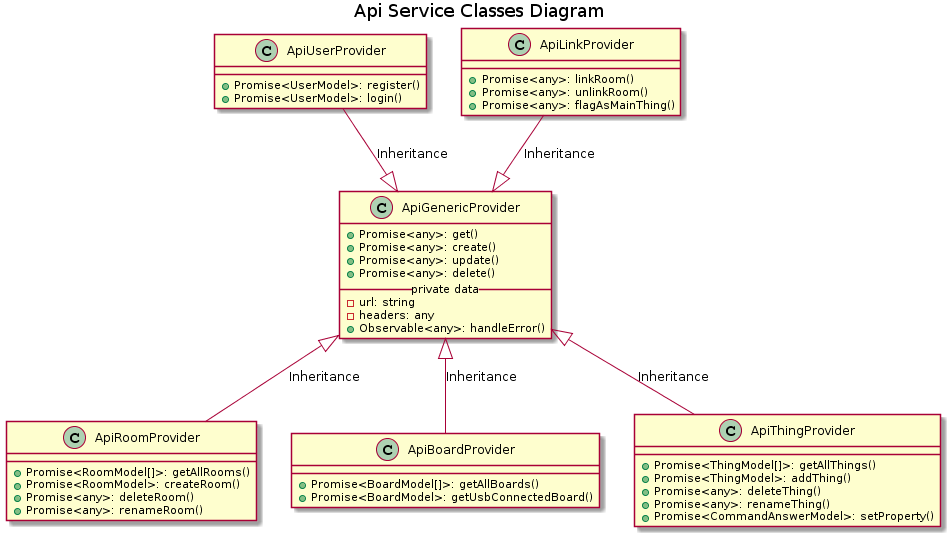
\includegraphics[height=2.5in]{figures/diagrams/front/architecture/api-services.png}
\caption[api-services]{api-services\footnotemark}
\end{figure}

\begin{figure}[hbt!]
\centering
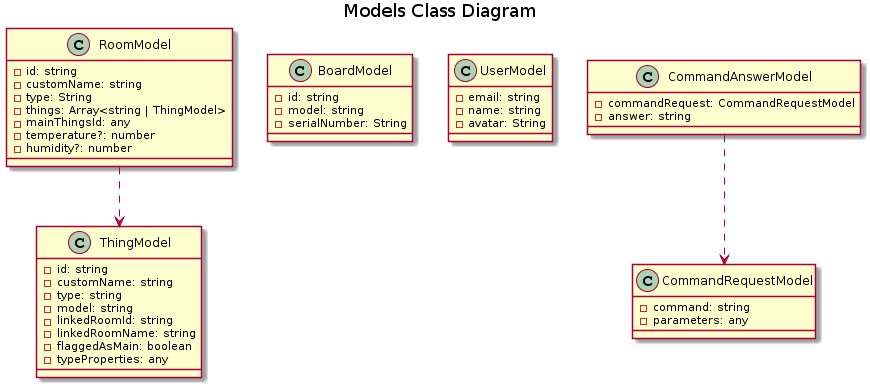
\includegraphics[height=2.5in]{figures/diagrams/front/architecture/models.png}
\caption[models]{models\footnotemark}
\end{figure}

\begin{figure}[hbt!]
\centering
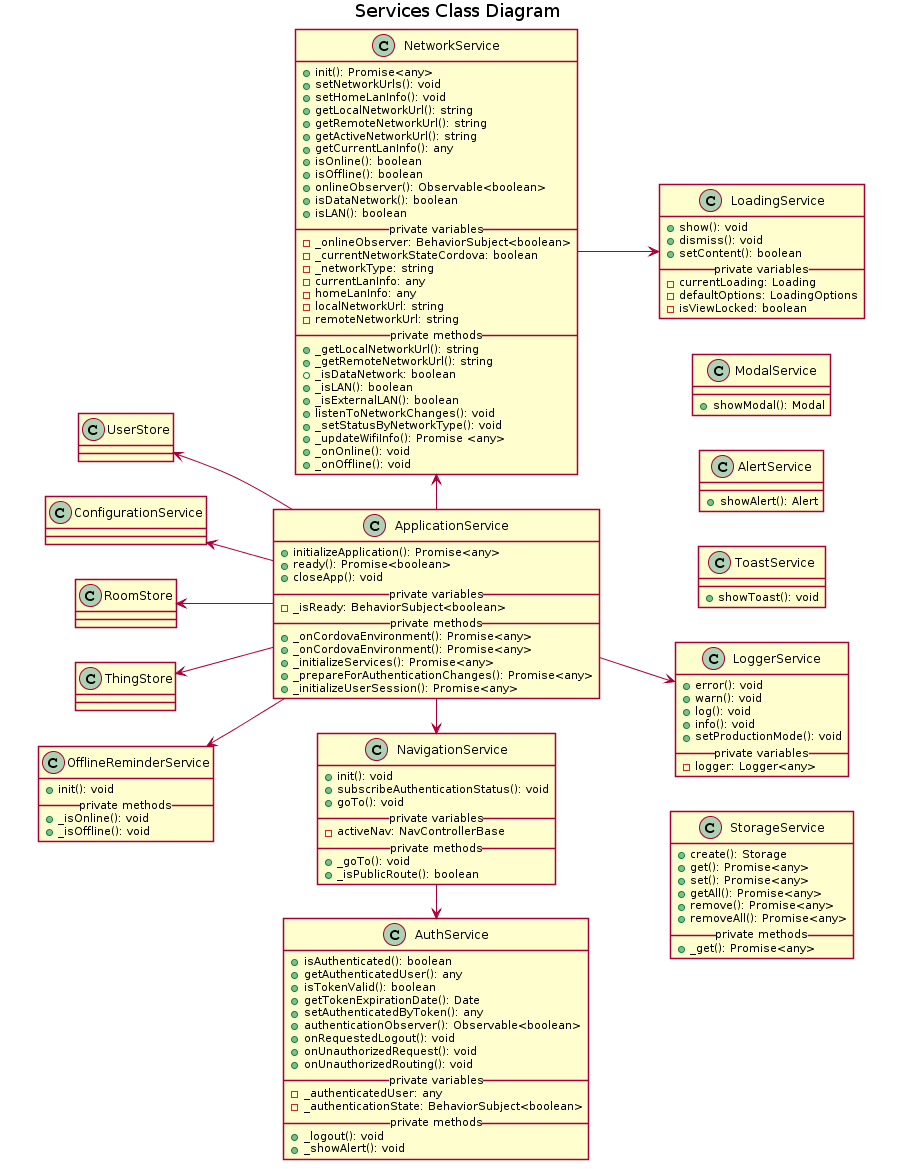
\includegraphics[height=2.5in]{figures/diagrams/front/architecture/services.png}
\caption[services]{services\footnotemark}
\end{figure}

\begin{figure}[hbt!]
\centering
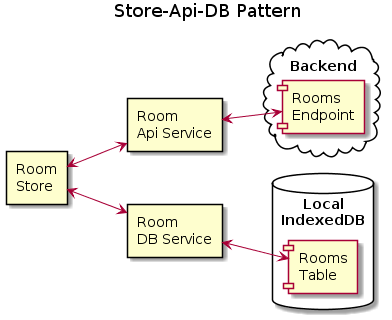
\includegraphics[height=2.5in]{figures/diagrams/front/architecture/store-api-db-pattern.png}
\caption[store-api-db-pattern]{store-api-db-pattern\footnotemark}
\end{figure}

\begin{figure}[hbt!]
\centering
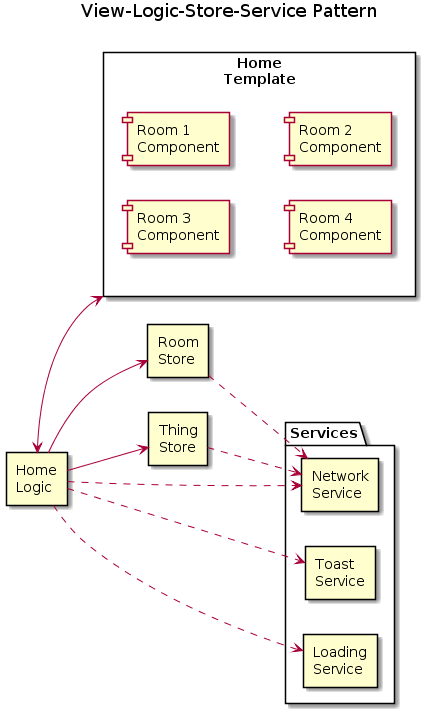
\includegraphics[height=2.5in]{figures/diagrams/front/architecture/view-logic-store-service-pattern.png}
\caption[view-logic-store-service-pattern]{view-logic-store-service-pattern\footnotemark}
\end{figure}

\begin{figure}[hbt!]
\centering
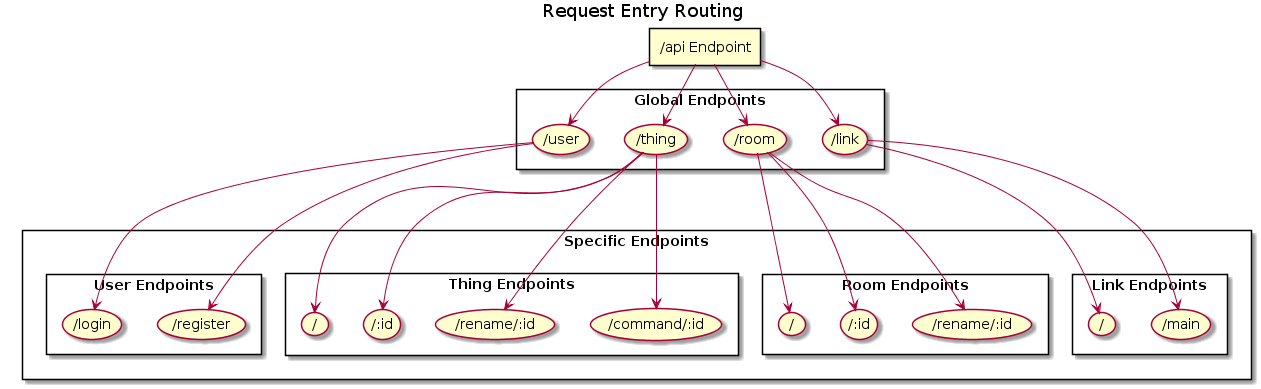
\includegraphics[height=2.5in]{figures/diagrams/back/router-flow/api-entry.png}
\caption[api-entry]{api-entry\footnotemark}
\end{figure}

\begin{figure}[hbt!]
\centering
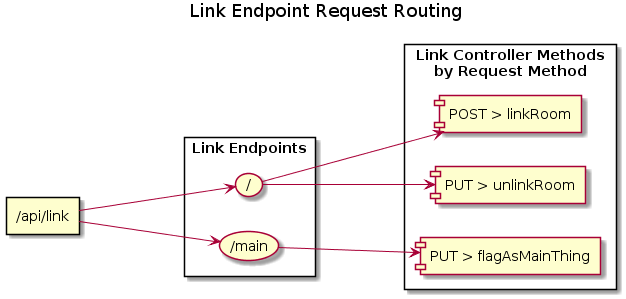
\includegraphics[height=2.5in]{figures/diagrams/back/router-flow/link-endpoints.png}
\caption[link-endpoints]{link-endpoints\footnotemark}
\end{figure}

\begin{figure}[hbt!]
\centering
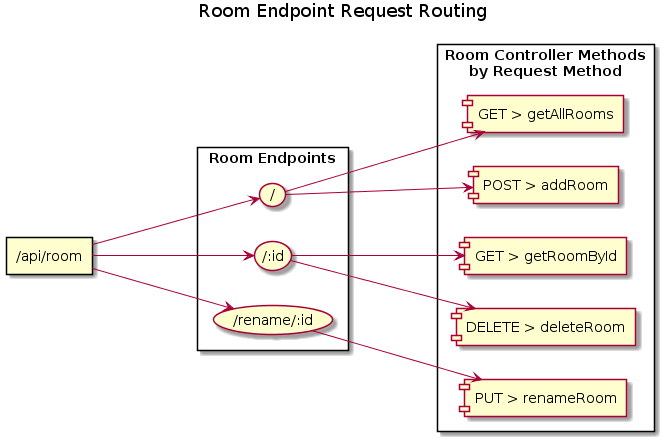
\includegraphics[height=2.5in]{figures/diagrams/back/router-flow/room-endpoints.png}
\caption[room-endpoints]{room-endpoints\footnotemark}
\end{figure}

\begin{figure}[hbt!]
\centering
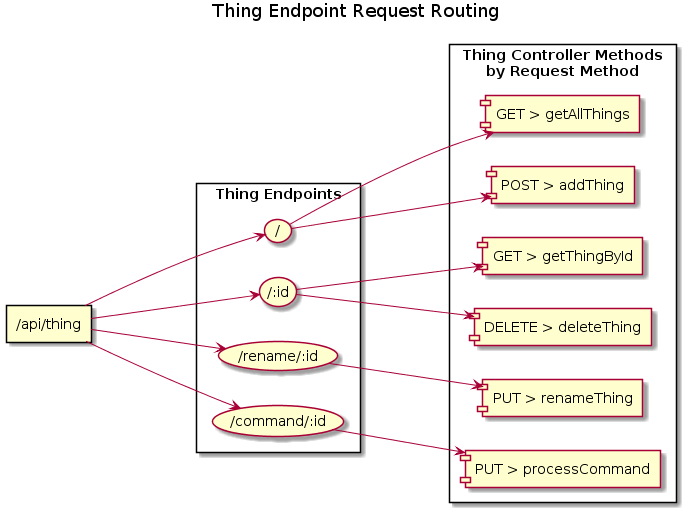
\includegraphics[height=2.5in]{figures/diagrams/back/router-flow/thing-endpoints.png}
\caption[thing-endpoints]{thing-endpoints\footnotemark}
\end{figure}

\begin{figure}[hbt!]
\centering
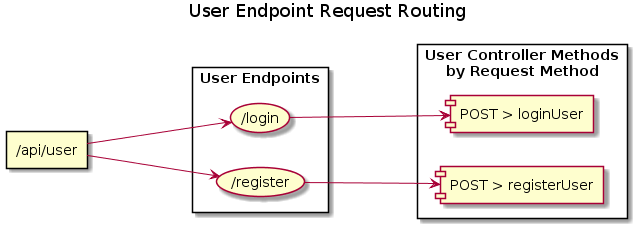
\includegraphics[height=2.5in]{figures/diagrams/back/router-flow/user-endpoints.png}
\caption[user-endpoints]{user-endpoints\footnotemark}
\end{figure}